\documentclass[11pt,a4paper]{report}

\usepackage[T1]{fontenc}
\usepackage{amsmath}
\usepackage{graphicx}
\usepackage[margin=1in]{geometry}
\usepackage{parskip}
\usepackage{xcolor}
\usepackage{booktabs}
\usepackage{array}
\usepackage{listings}
\usepackage{enumitem}
\usepackage{caption}
\usepackage{tikz}
\usetikzlibrary{positioning, arrows.meta, shapes.geometric}
\usepackage[hidelinks]{hyperref}

\definecolor{codebg}{gray}{0.95}
\definecolor{accent}{RGB}{30,80,140}
\definecolor{boxgreen}{RGB}{225,245,225}
\definecolor{boxred}{RGB}{250,225,225}
\definecolor{boxorange}{RGB}{252,235,215}
\definecolor{boxblue}{RGB}{228,230,248}

\hypersetup{colorlinks=true, linkcolor=black, urlcolor=accent, citecolor=black}

\lstset{
  basicstyle=\ttfamily\small,
  backgroundcolor=\color{codebg},
  frame=single,
  rulecolor=\color{gray!40},
  framesep=5pt,
  breaklines=true,
  columns=fullflexible,
  keepspaces=true,
  showstringspaces=false,
  xleftmargin=4pt,
  aboveskip=8pt,
  belowskip=8pt,
}

\newcommand{\code}[1]{\texttt{#1}}
\setlist{itemsep=2pt, topsep=4pt}
\captionsetup{font=small, labelfont=bf}

\begin{document}

%======================= TITLE PAGE =======================
\begin{titlepage}
\centering
\vspace*{0.6cm}
{\Large\textbf{Tribhuvan University}}\\[0.2cm]
{\large Institute of Engineering}\\[0.2cm]
{\large Pulchowk Campus}\\[0.8cm]


\includegraphics[width=3.2cm]{t.png}\\[0.8cm]

{\large\textbf{Final Project Report}}\\[0.4cm]
{\large On}\\[0.6cm]
{\Huge\textbf{GoBalancer}}\\[0.3cm]
{\large A Concurrent L4/L7 Load Balancer Written in Go}\\[1.8cm]

\textbf{Submitted By:}\\[0.3cm]
\begin{tabular}{ll}
Prabesh Bastola & (PUL080BCT052)\\
Sachin K.C.     & (PUL080BCT070)\\
Satyam Lamsal   & (PUL080BCT078)\\
\end{tabular}\\[1.8cm]

\textbf{Submitted To:}\\[0.3cm]
Department of Electronics and Computer Engineering\\
Subject: Network and System Programming\\
Instructor: Prabin Dhakal\\[1.8cm]

\textbf{August 2026}
\end{titlepage}

\pagenumbering{roman}

%======================= DECLARATION =======================
\chapter*{Declaration}
\addcontentsline{toc}{chapter}{Declaration}
We hereby declare that the work presented in this report titled \emph{GoBalancer: A
Concurrent L4/L7 Load Balancer Written in Go} is our own work, carried out for the subject
Network and System Programming. All sources of information and prior work used in this
project have been duly acknowledged. The design, implementation, testing, and results
reported here are the outcome of our own effort, and this report has not been submitted
elsewhere for any other purpose.

\vspace{1.5cm}
\noindent
\begin{tabular}{ll}
Prabesh Bastola (PUL080BCT052) & \hspace{3cm}\dotfill\\[0.8cm]
Sachin K.C. (PUL080BCT070)     & \hspace{3cm}\dotfill\\[0.8cm]
Satyam Lamsal (PUL080BCT078)   & \hspace{3cm}\dotfill\\
\end{tabular}

%======================= APPROVAL =======================
\chapter*{Approval}
\addcontentsline{toc}{chapter}{Approval}
This is to certify that the project titled \emph{GoBalancer: A Concurrent L4/L7 Load
Balancer Written in Go} has been examined and approved as partial fulfilment of the
requirements for the subject Network and System Programming, Department of Electronics and
Computer Engineering, Pulchowk Campus.

\vspace{2.5cm}
\noindent
\makebox[7cm]{\dotfill}\\
Prabin Dhakal\\
Instructor, Network and System Programming\\
Department of Electronics and Computer Engineering

%======================= COPYRIGHT =======================
\chapter*{Copyright}
\addcontentsline{toc}{chapter}{Copyright}
The authors grant the Department of Electronics and Computer Engineering, Pulchowk Campus,
permission to make this report freely available for inspection. The authors reserve other
publication rights, and neither the report nor extensive extracts from it may be reproduced
without the authors' written permission. The source code of GoBalancer is released as open
source and is available at \url{https://github.com/Sachinxmpl/gobalancer}.

%======================= ABSTRACT =======================
\chapter*{Abstract}
\addcontentsline{toc}{chapter}{Abstract}
GoBalancer is a load balancer implemented in Go that distributes client traffic across a
pool of backend servers. It operates in two modes: Layer~4 (TCP), a transparent byte-stream
proxy compatible with any TCP-based protocol, and Layer~7 (HTTP/HTTPS), a reverse proxy
capable of path- and header-aware routing. The system provides a unified load-balancing
interface with four algorithms --- Round Robin, Smooth Weighted Round Robin, Least
Connections, and Consistent Hashing with virtual nodes --- together with a two-plane
health-checking system, automatic failover with request retry, TLS termination with hot
certificate rotation, zero-downtime configuration reload, token-bucket rate limiting, and
Prometheus/Grafana observability.

The project was evaluated against five measurable goals: no goroutine leaks under fault
conditions, no dropped in-flight requests during reload and shutdown, sub-second failover,
live observability, and a reproducible benchmark report. The measured results show that the
proxy adds under half a millisecond of latency per request, scales linearly and cheaply to
ten thousand concurrent connections (under 200~MB of memory), moves only $1/N$ of keys when a
backend is removed under consistent hashing, and serves every client request with no error
burst across repeated backend failures. Chaos testing revealed three real correctness bugs
in the failover path, which were diagnosed and fixed; the debugging process itself is
documented as a contribution of this work.

%======================= ACKNOWLEDGEMENTS =======================
\chapter*{Acknowledgements}
\addcontentsline{toc}{chapter}{Acknowledgements}
We would like to express our sincere gratitude to our instructor, Prabin Dhakal, for his
guidance throughout this project, and to the Department of Electronics and Computer
Engineering, Pulchowk Campus, for providing the opportunity to undertake it. We are also
grateful to the open-source community whose tools --- the Go programming language, Prometheus,
Grafana, and Docker --- made this work possible.

%======================= FRONT LISTS =======================
\clearpage
\tableofcontents
\clearpage
\listoffigures
\listoftables

%======================= ABBREVIATIONS =======================
\chapter*{Abbreviations}
\addcontentsline{toc}{chapter}{Abbreviations}
\begin{tabbing}
\hspace{3cm}\= \kill
\textbf{L4} \> Layer 4 (transport layer, TCP)\\
\textbf{L7} \> Layer 7 (application layer, HTTP)\\
\textbf{TCP} \> Transmission Control Protocol\\
\textbf{HTTP} \> Hypertext Transfer Protocol\\
\textbf{HTTPS} \> HTTP Secure\\
\textbf{TLS} \> Transport Layer Security\\
\textbf{RR} \> Round Robin\\
\textbf{WRR} \> Weighted Round Robin\\
\textbf{XFF} \> X-Forwarded-For (HTTP header)\\
\textbf{SNI} \> Server Name Indication\\
\textbf{RPS} \> Requests Per Second\\
\textbf{RSS} \> Resident Set Size (process memory)\\
\textbf{GC} \> Garbage Collection\\
\textbf{LRU} \> Least Recently Used\\
\textbf{FNV} \> Fowler--Noll--Vo (hash function)\\
\textbf{RTT} \> Round-Trip Time\\
\textbf{CI} \> Continuous Integration\\
\textbf{YAML} \> YAML Ain't Markup Language\\
\textbf{p50/p99} \> 50th / 99th percentile latency\\
\end{tabbing}

%######################## CHAPTER 1 ########################
\clearpage
\pagenumbering{arabic}
\chapter{Introduction}

\section{Background}
Modern network services rarely run on a single server. To handle load and to survive
individual failures, a service is deployed as a pool of identical backend servers, and a
\emph{load balancer} sits in front of that pool. The load balancer presents a single stable
address to clients and spreads incoming traffic across the backends. This gives a service
three things a single server cannot provide: aggregate capacity, high availability (traffic
moves away from a failed backend), and a stable entry point that hides the changing set of
backends behind it.

Load balancers can operate at different layers of the network stack. A \emph{Layer~4} balancer
works at the transport layer and forwards raw TCP connections without inspecting the data
inside them; it is fast and protocol-agnostic. A \emph{Layer~7} balancer works at the
application layer, understands HTTP, and can therefore make richer routing decisions based on
the request path, headers, or cookies, at the cost of parsing every request. GoBalancer
implements both, so that the trade-off between the two can be studied directly.

Building such a system exercises the core of network and systems programming: socket
programming, safe concurrency across thousands of simultaneous connections, fault detection
and recovery, and operational concerns such as configuration reload, graceful shutdown, and
monitoring.

\section{Problem Statement}
Without a load balancer, client requests cannot be distributed across multiple backends, and
the failure of a single backend can reduce the availability of the entire service. A correct
load balancer must therefore solve several hard problems at once. It must handle many
concurrent connections without leaking resources; it must detect a failed backend quickly and
stop sending it traffic, yet readmit it carefully once it recovers; it must survive
configuration changes and its own shutdown without dropping in-flight requests; and it must do
all of this with low, predictable overhead. The problem this project addresses is to design
and implement such a load balancer, and to \emph{prove}, with measurements rather than
assertions, that it meets these requirements.

\section{Objectives}
\subsection{General Objective}
To design, implement, and evaluate a concurrent, production-style load balancer in Go that
distributes client traffic across a pool of backend servers while maintaining high
availability, efficient resource use, and fault tolerance.

\subsection{Specific Objectives}
The project is evaluated against five specific, measurable objectives:
\begin{description}[style=nextline,leftmargin=1.2cm]
  \item[G1 --- Correct concurrency (no leaks)] The goroutine count returns to its baseline
  after a sustained chaos test, verified by sampling and by pprof goroutine profiles.
  \item[G2 --- Zero dropped in-flight requests] Shutdown (\code{SIGTERM}) and reload
  (\code{SIGHUP}) under sustained load complete all already-accepted requests.
  \item[G3 --- Fast failover] When a backend is killed under load, the client-visible
  disruption window is under one second.
  \item[G4 --- Observability] Prometheus metrics and a Grafana dashboard make a backend's
  failure and recovery visible within one probe interval.
  \item[G5 --- Reproducible performance characterization] A benchmark report with throughput,
  latency percentiles, and scaling data, all reproducible via \code{make bench}.
\end{description}

\section{Rationale}
The project follows three design principles. First, \textbf{quality over quantity}: a smaller
set of features implemented correctly and tested thoroughly is worth more than many features
that merely appear to work. Second, \textbf{everything should be measurable}: every important
design decision is backed by a benchmark, a profile, or a test rather than an assumption.
Third, \textbf{incremental development}: the system was built in phases, each ending in a
working, demonstrable program. These principles make the final result trustworthy --- each
claim in this report can be re-checked by running the corresponding command.

\section{Scope}
The project delivers a single load-balancer process supporting both L4 and L7 modes, all four
balancing algorithms, the two-plane health system, TLS termination with reload-based
certificate rotation, hot configuration reload, rate limiting, Prometheus metrics with a
Grafana dashboard, a chaos-testing harness, and a reproducible benchmark suite. Backends are
declared in a YAML configuration file. A Docker Compose stack runs the balancer together with
demo backends and the monitoring stack.

\section{Limitations}
The following are intentionally out of scope: HTTP/2 and gRPC to backends; service discovery
via external systems such as Consul or etcd (backends are declared in the config file);
running multiple cooperating load-balancer instances for high availability; and rate limiting
shared across machines. In addition, all benchmarks are single-machine over loopback, so they
measure the balancer's own overhead rather than real-world network behaviour, and the active
health probe checks TCP connectivity only.

\section{Outline of the Report}
Chapter~2 reviews the relevant theory and existing systems. Chapter~3 describes the
methodology --- the project approach, system architecture, module design, technology stack,
and testing strategy. Chapter~4 covers implementation in detail, including the requirements,
the core algorithms and mechanisms, and the challenges faced. Chapter~5 presents the results
and discusses them, including comparative analysis. Chapter~6 concludes and lists future
enhancements.

%######################## CHAPTER 2 ########################
\chapter{Literature Review}

\section{Review of Related Theory}

\textbf{Layer 4 versus Layer 7 load balancing.} The two operating modes work with different
information and therefore offer different capabilities, summarised in Table~\ref{tab:l4l7}. L4
forwards TCP connections with minimal processing; L7 parses HTTP and can route on request
content.

\begin{table}[htbp]
\centering
\caption{Comparison of Layer 4 and Layer 7 load balancing.}
\label{tab:l4l7}
\begin{tabular}{p{3cm}p{5cm}p{5cm}}
\toprule
\textbf{Aspect} & \textbf{L4 (TCP)} & \textbf{L7 (HTTP)}\\
\midrule
Visible information & Source/destination IP and ports & Method, URL, headers, cookies\\
Routing unit & One backend per TCP connection & One backend per HTTP request\\
Protocols & Any TCP-based protocol & HTTP and HTTPS only\\
Balancing key & Usually client IP & Client IP, path, header, or cookie\\
Overhead & Minimal (direct forwarding) & Higher (requests are parsed)\\
Failure detection & Connection failures only & Connection failures and HTTP status\\
TLS & Encrypted traffic forwarded as-is & Can be terminated at the balancer\\
\bottomrule
\end{tabular}
\end{table}

\textbf{Consistent hashing.} A naive $\text{hash}(key) \bmod N$ mapping reassigns nearly every
key when $N$ changes. Consistent hashing, introduced by Karger et al.~\cite{karger}, places
both backends and keys on a ring so that adding or removing one backend reassigns only about
$1/N$ of the keys. Virtual nodes (multiple ring positions per backend) smooth out the
distribution. This makes it the standard choice for cache affinity and sticky sessions.

\textbf{Smooth weighted round robin.} A naive weighted scheme sends a burst of consecutive
requests to a heavier backend. The smooth weighted round-robin algorithm, popularised by
nginx~\cite{nginx}, interleaves picks by tracking a running ``current weight'' per backend,
producing a smoother distribution.

\textbf{Health checking.} Production systems combine \emph{active} probing with \emph{passive}
observation of real traffic; the asymmetric ``evict quickly, readmit slowly'' policy mirrors
outlier-detection features in Envoy and HAProxy~\cite{envoy}.

\textbf{Concurrency and the Go netpoller.} Go schedules many goroutines onto a small number of
OS threads and parks a goroutine that is waiting on network I/O using an event notification
mechanism (\code{epoll} on Linux)~\cite{netpoll}. A goroutine starts with a small stack (a few
kilobytes), so a goroutine-per-connection design remains practical at thousands of
connections.

\textbf{Coordinated omission.} Tene~\cite{tene} shows that a load generator which waits for
each reply before sending the next one hides latency during stalls. Correct latency
measurement requires an open-loop, constant-rate generator --- a principle this project's
benchmark methodology follows.

\section{Review of Related Works}
Several mature load balancers informed this design:
\begin{itemize}
  \item \textbf{NGINX} --- a widely deployed reverse proxy and L7 load balancer; the source of
  the smooth weighted round-robin algorithm used here.
  \item \textbf{HAProxy} --- a high-performance L4/L7 balancer known for its health-checking and
  observability; its \code{rise}/\code{fall} probe semantics are adopted directly.
  \item \textbf{Envoy} --- a modern service-mesh proxy whose outlier-detection model
  (passive ejection plus active checks) matches the two-plane health design.
  \item \textbf{Traefik} --- a Go-based reverse proxy and load balancer, demonstrating that the
  goroutine-per-connection model scales in practice.
\end{itemize}
Table~\ref{tab:related} places GoBalancer alongside these systems.

\begin{table}[htbp]
\centering
\caption{GoBalancer in relation to existing load balancers.}
\label{tab:related}
\begin{tabular}{p{3.5cm}cccc}
\toprule
\textbf{Feature} & \textbf{NGINX} & \textbf{HAProxy} & \textbf{Envoy} & \textbf{GoBalancer}\\
\midrule
L4 and L7 modes        & partial & yes & yes & yes\\
Consistent hashing     & yes & yes & yes & yes\\
Active + passive health& yes & yes & yes & yes\\
Hot reload             & yes & yes & yes & yes\\
Written in Go          & no  & no  & no  & yes\\
Scope                  & large & large & large & focused / educational\\
\bottomrule
\end{tabular}
\end{table}

\section{Gap Analysis}
The existing systems are large, mature, and written mostly in C or C++. They are excellent
tools but poor \emph{teaching artefacts}: their scale hides the core mechanisms. GoBalancer
fills a narrower gap --- a compact, readable, fully-tested load balancer written against the
Go standard library, where each mechanism (the lock-free data path, the health state machine,
the consistent-hash ring, the failover retry) is small enough to be understood, yet complete
enough to be measured against the same properties production systems care about. The
contribution is not a new algorithm but a correct, measured, and documented synthesis.

%######################## CHAPTER 3 ########################
\chapter{Methodology}

\section{Project Approach}
The system was built \emph{incrementally} across seven phases (P0--P6), each ending in a
working, demonstrable program with its own exit criterion. P0 established the skeleton (config
parsing, CI); P1 the L4 TCP proxy; P2 the health loop; P3 the L7 proxy and TLS; P4 the
remaining algorithms; P5 operations (reload, rate limiting, metrics, dashboard); and P6 the
chaos harness, benchmarks, and this report. Correctness goals (G1--G3) were treated as
non-negotiable: under schedule pressure, features would be cut before correctness tests.

\section{System Architecture}
The central architectural decision is a strict separation between a \emph{data plane} and a
\emph{control plane}. The data plane is the hot path --- accept a connection, pick a backend,
move bytes --- and must never block on administrative work. The control plane is the cold path
--- load and validate configuration, run health probes, react to signals --- and may use locks
freely. The two planes meet at exactly one point: an immutable configuration snapshot published
behind a single atomic pointer. Figure~\ref{fig:arch} shows the overall structure.

\begin{figure}[htbp]
\centering
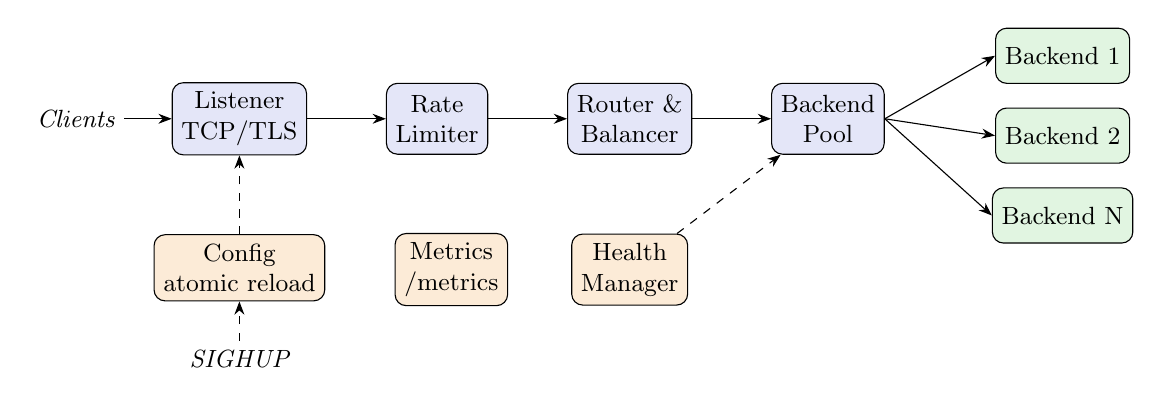
\begin{tikzpicture}[
  node distance=8mm and 10mm,
  box/.style={draw, rounded corners, align=center, minimum height=9mm, font=\small, fill=boxblue},
  be/.style={draw, rounded corners, align=center, minimum height=7mm, font=\small, fill=boxgreen},
  aux/.style={draw, rounded corners, align=center, minimum height=8mm, font=\small, fill=boxorange},
  ext/.style={draw, dashed, rounded corners, align=center, minimum height=7mm, font=\small},
  >={Stealth[]},
]
\node[box] (lis) {Listener\\TCP/TLS};
\node[box, right=of lis] (rl) {Rate\\Limiter};
\node[box, right=of rl] (rb) {Router \&\\Balancer};
\node[box, right=of rb] (bp) {Backend\\Pool};
\node[be, right=14mm of bp, yshift=8mm] (b1) {Backend 1};
\node[be, below=3mm of b1] (b2) {Backend 2};
\node[be, below=3mm of b2] (bn) {Backend N};

\node[aux, below=10mm of lis] (cfg) {Config\\atomic reload};
\node[aux, below=10mm of rb] (hm) {Health\\Manager};
\node[aux, left=8mm of hm] (mx) {Metrics\\/metrics};

\draw[->] (lis) -- (rl);
\draw[->] (rl) -- (rb);
\draw[->] (rb) -- (bp);
\draw[->] (bp.east) -- (b1.west);
\draw[->] (bp.east) -- (b2.west);
\draw[->] (bp.east) -- (bn.west);
\draw[dashed,->] (cfg) -- (lis);
\draw[dashed,->] (hm) -- (bp);
\node[left=6mm of lis, font=\small\itshape] (cl) {Clients};
\draw[->] (cl) -- (lis);
\node[below=5mm of cfg, font=\small\itshape] (hup) {SIGHUP};
\draw[dashed,->] (hup) -- (cfg);
\end{tikzpicture}
\caption{High-level architecture of GoBalancer. Solid arrows are the client-request path;
dashed arrows are configuration updates and monitoring.}
\label{fig:arch}
\end{figure}

\section{System Design and Modules}
The balancer is divided into independent modules, each with one responsibility:
\begin{itemize}
  \item \textbf{Listener} --- accepts incoming TCP or TLS connections.
  \item \textbf{Rate Limiter} --- enforces global and per-client request limits.
  \item \textbf{Router and Balancer} --- selects the backend pool (by path in L7) and picks a
  healthy backend using the configured algorithm.
  \item \textbf{Backend Pool / Registry} --- holds each backend's health state and live
  connection count, outside the config snapshot so it survives reloads.
  \item \textbf{Health Manager} --- runs one prober per backend, evicting and readmitting
  backends through the state machine.
  \item \textbf{Configuration Manager} --- loads, validates, and atomically swaps the config.
  \item \textbf{Metrics System} --- exports Prometheus metrics on a separate port.
\end{itemize}

\section{Technology Stack}
The implementation targets Go~1.26 and deliberately limits itself to four runtime
dependencies, relying on the standard library for everything else. The stack is summarised in
Table~\ref{tab:stack}.

\begin{table}[htbp]
\centering
\caption{Technology stack.}
\label{tab:stack}
\begin{tabular}{ll}
\toprule
\textbf{Concern} & \textbf{Choice}\\
\midrule
Language & Go 1.26\\
Config parsing & \code{gopkg.in/yaml.v3}\\
Rate limiting & \code{golang.org/x/time/rate}\\
Metrics & \code{prometheus/client\_golang}\\
Optional file watch & \code{fsnotify}\\
Leak detection (test) & \code{go.uber.org/goleak}\\
Containerisation & Docker, Docker Compose\\
Monitoring & Prometheus, Grafana\\
Profiling & \code{net/http/pprof}\\
\bottomrule
\end{tabular}
\end{table}

\section{Development Methodology}
Development followed an incremental, test-driven process. Each package carries unit tests run
under the race detector, and continuous integration runs formatting checks, \code{go vet},
and the full test suite on every change. Work was tracked in phases, each merged only once its
exit criterion was met.

\section{Data Handling}
There are three kinds of data in the system. \emph{Configuration} is read from a YAML file,
validated, and held as an immutable snapshot behind an atomic pointer; a reload builds a new
snapshot and swaps it. \emph{Request and response bodies} are streamed, never fully buffered,
so that large payloads do not inflate memory. \emph{Operational data} (per-backend health and
connection counts, metric counters) lives in small concurrent structures --- atomic counters on
the hot path, a mutex only where state genuinely changes.

\section{Testing and Validation}
Validation uses five complementary techniques: unit tests with the race detector; goroutine-leak
detection with \code{goleak}; differential (equivalence) testing of the L7 proxy against the
standard library's \code{httputil.ReverseProxy}; a chaos harness that kills backends under load;
and a reproducible benchmark suite. These map directly onto the goals: the chaos harness proves
G1 and G3, the reload and drain tests prove G2, the dashboard proves G4, and the benchmark suite
proves G5.

\section{Deployment Setup}
Two deployment paths are used. For demonstration and chaos testing, a Docker Compose stack runs
the balancer, three demo backends, Prometheus, and a preloaded Grafana dashboard; the balancer
is built as a static binary into a \code{scratch} image via a multi-stage Dockerfile. For
benchmarking, the components run as bare host processes over loopback, so that measurements
reflect the balancer rather than Docker's virtual network.

%######################## CHAPTER 4 ########################
\chapter{Implementation Details}

\section{Requirements Specification}
\textbf{Functional requirements.} The system shall: forward TCP connections (L4) and HTTP(S)
requests (L7); select a backend using any of four configurable algorithms; route L7 requests to
a pool by longest matching path prefix; detect a failed backend and remove it from rotation;
readmit a recovered backend after successful probes; retry a failed idempotent request on
another backend; terminate TLS and rotate certificates on reload; reload configuration on
\code{SIGHUP} without dropping connections; enforce global and per-client rate limits; and export
Prometheus metrics.

\textbf{Non-functional requirements.} The system shall add sub-millisecond latency on the hot
path; scale to at least ten thousand concurrent connections without leaking resources; never drop
an accepted request during reload or shutdown; and keep metric cardinality bounded.

\textbf{Constraints.} At most four runtime dependencies; Go~1.26; Linux as the primary platform.

\section{System Overview}
The methodology of Chapter~3 maps onto concrete Go packages: a \code{config} package (parse,
validate, atomic \code{Store}); a \code{balancer} package (the four algorithms behind a common
\code{Pick} interface); a \code{health} package (the registry, state machine, and prober
manager); \code{proxy/l4} and \code{proxy/l7} packages (the two data paths); a \code{ratelimit}
package; a \code{reload} package; and a \code{metrics} package. A request reads the config
snapshot once and flows through these packages without acquiring a lock on the hot path.

\section{Development Environment}
The system was developed and measured on the environment in Table~\ref{tab:env}.

\begin{table}[htbp]
\centering
\caption{Development and measurement environment.}
\label{tab:env}
\begin{tabular}{ll}
\toprule
CPU & 13th Gen Intel Core i5-13420H (12 cores)\\
Memory & 15 GiB\\
OS & Linux (Pop!\_OS, kernel 7.0.11)\\
Go toolchain & go1.26.5\\
\bottomrule
\end{tabular}
\end{table}

\section{System Implementation}

\subsection{The request pipeline}
For an L7 request the pipeline is: (1)~rate-limit check; (2)~load the config snapshot with one
atomic read; (3)~route to a pool by longest matching path prefix; (4)~filter the pool to healthy
backends; (5)~pick one backend by the configured algorithm; (6)~forward, retrying on another
healthy backend if the connection fails; (7)~stream the response back. In L4 mode the pipeline is
similar but the ``request'' is the whole TCP stream, selected once and relayed byte-for-byte.

\subsection{L4 --- the TCP relay}
An accepted connection uses three goroutines: one owning the connection plus one for each
direction of an \code{io.Copy}. The tricky part is closing correctly: when one direction ends,
the code half-closes that side (\code{CloseWrite}, sending an EOF) so the other direction can
finish, applies a deadline so a stalled peer cannot hold the connection forever, and only then
closes both sides and decrements the connection count. Getting this wrong is the classic source
of goroutine leaks, which is why it is exercised directly by the chaos test.

\subsection{L7 --- correct HTTP forwarding}
Forwarding an HTTP request correctly means obeying four rules: clear the incoming
\code{RequestURI} before reusing the request outbound; strip hop-by-hop headers (\code{Connection},
\code{Keep-\allowbreak Alive}, \code{Transfer-\allowbreak Encoding}, and any names listed inside \code{Connection});
append the client IP to \code{X-Forwarded-For}; and stream the body. Backend connections are
pooled through a shared \code{http.Transport}. A key setting is \code{ResponseHeaderTimeout},
fixed at 300~ms: it bounds how long a pooled connection to a silently-dead backend waits before
failing. Rather than use the standard library's \code{httputil.ReverseProxy}, GoBalancer
implements the proxy directly for control over these rules, and validates the result against the
library proxy (Section~\ref{sec:testing-impl}).

\subsection{The four algorithms}
\textbf{Round Robin} uses a single atomic counter modulo the pool size --- cheapest, even by
count, blind to load. \textbf{Smooth Weighted Round Robin} tracks a running current weight per
backend under a small lock, interleaving picks so a 3:1 weighting yields
\code{A B A C A B A C}. \textbf{Least Connections} picks the backend with the fewest in-flight
requests (each backend carries an atomic counter incremented on dispatch and decremented on
completion), breaking ties with round robin; it naturally steers away from a slow backend whose
counter stays high. \textbf{Consistent Hashing} builds a ring with 150 virtual nodes per backend
using an FNV-1a hash, published immutably behind an atomic pointer and rebuilt only when the
pool's membership fingerprint changes; a key maps to the first backend clockwise from its hash,
so removing a backend disturbs only its own keys.

\subsection{The health state machine}
Each backend moves through four phases --- Healthy, Evicted, Cooldown, Probation ---
following the policy ``fail fast, recover carefully'' (Figure~\ref{fig:health}). The passive
path is the only mechanism that evicts (after \code{fall} consecutive real-traffic failures);
the active prober is the only mechanism that readmits (after a cooldown and \code{rise}
consecutive successful probes). The registry keeps this state outside the config snapshot, and a
reload reconciles rather than rebuilds it. Table~\ref{tab:health} lists the default parameters.

\begin{figure}[htbp]
\centering
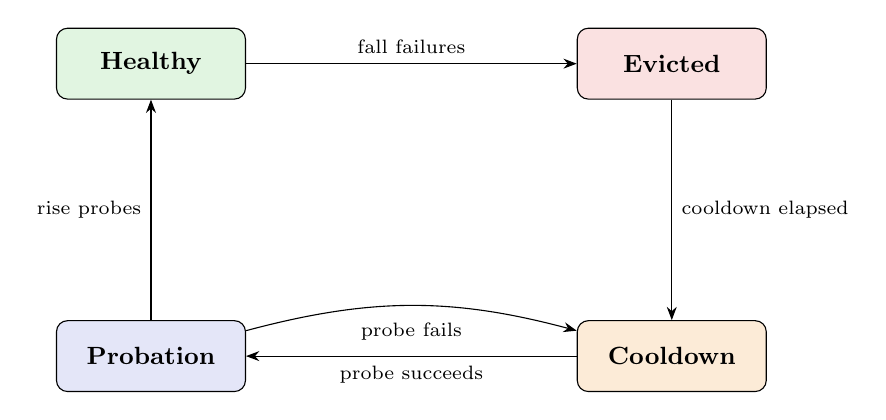
\begin{tikzpicture}[
  node distance=28mm and 42mm,
  st/.style={draw, rounded corners, minimum width=24mm, minimum height=9mm, font=\small\bfseries},
  >={Stealth[]}, font=\small,
]
\node[st, fill=boxgreen] (h) {Healthy};
\node[st, fill=boxred, right=of h] (e) {Evicted};
\node[st, fill=boxorange, below=of e] (c) {Cooldown};
\node[st, fill=boxblue, below=of h] (p) {Probation};
\draw[->] (h) -- node[above,font=\scriptsize]{fall failures} (e);
\draw[->] (e) -- node[right,font=\scriptsize]{cooldown elapsed} (c);
\draw[->] (c) -- node[below,font=\scriptsize]{probe succeeds} (p);
\draw[->] (p) -- node[left,font=\scriptsize]{rise probes} (h);
\draw[->] (p) to[bend left=15] node[below,font=\scriptsize,yshift=-1mm]{probe fails} (c);
\end{tikzpicture}
\caption{Backend health state machine. Eviction is immediate; recovery requires a cooldown and
several consecutive good probes.}
\label{fig:health}
\end{figure}

\begin{table}[htbp]
\centering
\caption{Default health-check parameters (all configurable).}
\label{tab:health}
\begin{tabular}{lll}
\toprule
\textbf{Parameter} & \textbf{Default} & \textbf{Role}\\
\midrule
fall (failure threshold) & 3 & passive: failures before eviction\\
cooldown & 10s & wait after eviction before probing\\
rise (success threshold) & 2 & active: good probes before readmit\\
probe interval & 2s & active: time between probes\\
probe timeout & 500ms & active: max wait for a probe\\
\bottomrule
\end{tabular}
\end{table}

\subsection{Failover with retry}
When a connection-level failure occurs and the client has not itself disconnected, the request is
retried on a different healthy backend --- for idempotent methods only, across up to three
distinct backends, and only before any response byte has been written. This makes a dying backend
invisible to clients while the health system catches up.

\subsection{Configuration reload and TLS}
Reload follows a strict validate-before-swap discipline: on \code{SIGHUP} the new file is parsed
and validated completely, and only then is the config pointer swapped and the registry
reconciled; an invalid file is rejected and the running config is kept. TLS certificates are
resolved per handshake from the current snapshot, so certificate rotation is just a reload.

\subsection{Rate limiting and metrics}
Rate limiting uses token buckets at two levels (global and per-client-IP), with per-client
buckets in an LRU-bounded map so a flood of unique IPs cannot exhaust memory; over-limit traffic
is rejected immediately rather than queued. Metrics are exported on a separate port with bounded
cardinality --- labelled by status class and backend, never by exact code, client IP, or path.
Table~\ref{tab:metrics} lists the key series.

\begin{table}[htbp]
\centering
\caption{Key Prometheus metrics.}
\label{tab:metrics}
\begin{tabular}{lll}
\toprule
\textbf{Metric} & \textbf{Type} & \textbf{Purpose}\\
\midrule
request count & counter & requests by backend and status class\\
request duration & histogram & latency percentiles by backend\\
active connections & gauge & live connections per backend\\
backend up & gauge & health of each backend\\
health transitions & counter & evictions and readmissions\\
rate-limit rejections & counter & requests refused by the limiter\\
reload outcomes & counter & successful and failed reloads\\
\bottomrule
\end{tabular}
\end{table}

\section{Interface and Visualization}
GoBalancer is operated through a command-line interface (\code{run} and \code{check}
sub-commands) and a YAML configuration file (Appendix~A and~B). Live state is visualised through
a Grafana dashboard, provisioned automatically in the Docker stack, showing request rate and
latency, per-backend health and active connections, goroutine and memory usage, and rate-limit
and reload events. During a demonstration the dashboard shows a backend being killed, evicted,
and readmitted --- satisfying goal G4. Profiling data is available on demand through pprof
endpoints on a private debug port.

\section{Deployment and Execution}
The system is built with \code{make build} and run as \code{gobalancer run -c config.yaml}. The
full demonstration stack is started with \code{docker compose up --build}, exposing the proxy on
port 8080, metrics on 9095, and Grafana on 3000. Benchmarks run as bare processes via
\code{make bench}; the chaos harness runs via \code{bash test/chaos/run.sh}. All commands are
listed in Appendix~C.

\section{Challenges and Solutions}
\label{sec:testing-impl}
The most instructive part of the project was a set of correctness bugs in the failover path that
only surfaced under chaos testing, where killing backends under load initially produced
multi-second error windows and a goroutine count climbing from 14 into the hundreds. Three
distinct bugs were hiding behind that one symptom.

\textbf{Challenge 1: a client hang-up counted as a backend failure.} The proxy derived each
request's context from the incoming request. When a client gave up and closed its connection, that
context was cancelled, the outbound call returned an error, and the code recorded a backend
failure. Under load this evicted \emph{healthy} backends --- sometimes all of them at once,
producing 100\%-failure windows. \emph{Solution:} check whether the client's own context was
cancelled and, if so, do not blame the backend.

\textbf{Challenge 2: no retry.} Any connection failure returned \code{502} to the client
immediately, so every request that landed on a just-killed backend was a visible error.
\emph{Solution:} retry idempotent requests on another healthy backend before returning an error.

\textbf{Challenge 3: dead connections were never closed.} A dead backend's pooled connections
lingered until a 90-second idle timeout, each with a live goroutine, so the count climbed with
every kill. \emph{Solution:} close idle connections the moment a backend is evicted, and tighten
the pool.

Two further lessons: the \code{goleak} check must run through \code{TestMain}, not a deferred call
inside a test, or it races the test's own cleanup and reports false leaks; and the L7 latency
tax is sub-millisecond, so the benchmark generator had to record microseconds, not milliseconds,
to make it visible. Chaos testing did not just verify the system --- it \emph{found real bugs},
which is exactly its purpose.

%######################## CHAPTER 5 ########################
\chapter{Results and Discussion}

\section{Results}
All benchmarks ran as bare processes over loopback, driven by an open-loop constant-rate
generator, on the environment of Table~\ref{tab:env}. Each experiment is reproducible via
\code{make bench}.

\textbf{E1 --- Proxy overhead.} Latency direct versus through the proxy, at 1000 rps against a
5~ms backend (Table~\ref{tab:e1}). The proxy adds under half a millisecond; L7 costs about twice
L4.

\begin{table}[htbp]
\centering
\caption{E1: per-request overhead of the proxy.}
\label{tab:e1}
\begin{tabular}{lrrr}
\toprule
target & p50 & p99 & overhead (p50)\\
\midrule
direct     & 5.59\,ms & 6.46\,ms & ---\\
through L4 & 5.78\,ms & 6.60\,ms & +0.19\,ms\\
through L7 & 6.01\,ms & 7.01\,ms & +0.42\,ms\\
\bottomrule
\end{tabular}
\end{table}

\textbf{E2 --- Connection scaling.} Goroutines and memory versus live connections
(Table~\ref{tab:e2}). The goroutine count is exactly $12 + 3 \times \text{connections}$ ---
perfectly linear --- and 10{,}000 connections cost under 200~MB with zero failures.

\begin{table}[htbp]
\centering
\caption{E2: goroutine-per-connection scaling.}
\label{tab:e2}
\begin{tabular}{rrr}
\toprule
connections & goroutines & memory\\
\midrule
100   & 312   & 16.9\,MB\\
1000  & 3012  & 32.9\,MB\\
5000  & 15012 & 107.5\,MB\\
10000 & 30012 & 189.5\,MB\\
\bottomrule
\end{tabular}
\end{table}

\textbf{E3 --- Least-connections versus round-robin} with one slow backend
(Table~\ref{tab:e3}). Least-connections cuts mean latency by a factor of five by steering away
from the slow backend.

\begin{table}[htbp]
\centering
\caption{E3: algorithm behaviour with two 5\,ms and one 150\,ms backend.}
\label{tab:e3}
\begin{tabular}{lrrr}
\toprule
algorithm & p50 & p90 & mean\\
\midrule
round\_robin       & 6.5\,ms & 151\,ms & 54.7\,ms\\
least\_connections & 6.2\,ms & 6.9\,ms & 10.1\,ms\\
\bottomrule
\end{tabular}
\end{table}

\textbf{E4 --- Consistent-hash remap} (Table~\ref{tab:e4}). Removing one of ten backends moves
exactly $1/N$ of keys under consistent hashing, versus 90\% for naive modulo.

\begin{table}[htbp]
\centering
\caption{E4: fraction of keys moved when one of ten backends is removed.}
\label{tab:e4}
\begin{tabular}{lrr}
\toprule
method & keys moved (avg) & per-drop range\\
\midrule
consistent\_hash & 10.0\% & 4.3\%--16.0\%\\
modulo\_n        & 90.1\% & ---\\
\bottomrule
\end{tabular}
\end{table}

\textbf{E5 --- Value of the health loop} (Table~\ref{tab:e5}). With a sick backend, passive
eviction keeps the mean near 8~ms; disabling it lets a third of requests suffer the sick backend,
pushing the mean to 106~ms.

\begin{table}[htbp]
\centering
\caption{E5: latency with and without passive eviction, one sick backend.}
\label{tab:e5}
\begin{tabular}{lrrr}
\toprule
health & p50 & p90 & mean\\
\midrule
passive+active & 6.1\,ms & 6.7\,ms & 8.3\,ms\\
active-only    & 6.5\,ms & 307\,ms & 106\,ms\\
\bottomrule
\end{tabular}
\end{table}

\textbf{Profiling.} Under load the proxy used about 0.86 of one core; its CPU profile was
dominated by network syscalls and the goroutine scheduler, its live heap was under 4~MB, and its
goroutines all mapped to known roles --- the signature of a proxy that moves data rather than
computing.

\textbf{Chaos test.} Across ten backend kills under sustained load, every client request was
served, no error burst exceeded one second, and the goroutine count returned to baseline. The
harness confirms that the chaos actually occurred by counting evictions from the metrics.

\textbf{Goals.} Table~\ref{tab:goals} summarises the outcome against the five goals.

\begin{table}[htbp]
\centering
\caption{Results against the project goals.}
\label{tab:goals}
\begin{tabular}{cll}
\toprule
Goal & Status & Evidence\\
\midrule
G1 & Met & Chaos returns to baseline; \code{goleak} green in CI\\
G2 & Met & Reload and drain tests pass against the built binary\\
G3 & Met & Zero error burst across ten backend kills\\
G4 & Met & Live Grafana dashboard of backend state\\
G5 & Met & \code{make bench} reproduces all five experiments\\
\bottomrule
\end{tabular}
\end{table}

\section{Discussion}
The results confirm the design. The sub-millisecond overhead (E1) shows the lock-free data path
is not a bottleneck; the exact linearity of E2 confirms the goroutine-per-connection model holds
and that no per-connection resource leaks. E3 and E5 demonstrate that the adaptive algorithm and
the health loop each deliver a large, measurable reduction in tail latency under partial failure
--- the situations that matter most in practice. E4 verifies the theoretical $1/N$ property of
consistent hashing on the actual shipped ring. Together with the chaos result, the evidence shows
the system meets all five goals not by assertion but by measurement.

An honest limitation surfaced in E5: because the active prober checks only TCP connectivity, it
briefly readmits a backend that accepts connections but does not serve them, causing a small tail
(p999) even under the full health loop. An HTTP-level probe would close this gap and is noted as
future work.

\section{Comparative Analysis}
The comparative results follow directly from the experiments. \textbf{L4 versus L7:} L4 is
roughly twice as cheap as L7 (E1), because it copies bytes while L7 parses HTTP --- the expected
trade-off between speed and routing intelligence. \textbf{Least-connections versus round-robin:}
identical when all backends are healthy, but least-connections is five times better on mean
latency when one backend is slow (E3). \textbf{Consistent hashing versus modulo:} nine times
fewer keys move on a membership change (E4), the difference between a 10\% and a 90\%
cache-miss event. \textbf{Health loop on versus off:} the difference between an 8~ms and a 106~ms
mean under a sick backend (E5). In every comparison the more sophisticated choice pays for itself
precisely under failure, which is when a load balancer earns its keep.

%######################## CHAPTER 6 ########################
\chapter{Conclusions and Recommendations}

\section{Conclusions}
This project designed, implemented, and evaluated GoBalancer, a concurrent L4/L7 load balancer
written in Go against the standard library with only four runtime dependencies. All five
measurable goals were met: no goroutine leaks under sustained fault injection, no dropped
in-flight requests during reload and shutdown, sub-second failover, live observability, and a
fully reproducible benchmark report. The system adds under half a millisecond of latency per
request, scales linearly to ten thousand connections in under 200~MB, and routes correctly around
failed and slow backends.

Beyond the working system, the project demonstrates a methodology: every design decision is
backed by a measurement, and the chaos-testing process uncovered three genuine correctness bugs
in the failover path that ordinary unit tests missed. The lesson --- that resilience must be
tested by inducing failure, not assumed --- is itself a result of this work.

\section{Recommendations and Future Enhancements}
The following extensions are natural next steps:
\begin{itemize}
  \item \textbf{HTTP-level health probes} to detect backends that accept connections but do not
  serve, closing the gap found in E5.
  \item \textbf{SNI-based routing in L4 mode}, inspecting the TLS ClientHello to route by hostname
  while preserving end-to-end encryption.
  \item \textbf{HTTP/2 to backends} and WebSocket/upgrade support in L7 mode.
  \item \textbf{Weighted least-connections}, combining capacity weights with live load.
  \item \textbf{A stronger load generator} to characterise maximum throughput under saturation,
  complementing the latency-focused benchmarks.
  \item \textbf{Distributed operation} --- multiple cooperating instances and shared rate limiting
  --- for high availability beyond a single process.
\end{itemize}

%======================= REFERENCES =======================
\begin{thebibliography}{9}
\addcontentsline{toc}{chapter}{References}
\bibitem{gostd} Go standard library documentation: \code{net}, \code{net/http},
\code{net/http/httputil}, \code{crypto/tls}, \code{context}, \code{log/slog}, \code{hash/fnv}.
\url{https://pkg.go.dev}.
\bibitem{karger} D. Karger, E. Lehman, T. Leighton, R. Panigrahy, M. Levine, and D. Lewin,
``Consistent Hashing and Random Trees: Distributed Caching Protocols for Relieving Hot Spots on
the World Wide Web,'' in \emph{Proc. 29th ACM Symposium on Theory of Computing (STOC)}, 1997.
\bibitem{nginx} nginx development team, upstream module: smooth weighted round-robin balancing.
\url{https://github.com/nginx/nginx}.
\bibitem{envoy} Envoy Proxy documentation, ``Outlier Detection''; HAProxy Configuration Manual,
\code{observe}, \code{rise}, \code{fall} directives --- prior art for the asymmetric evict/readmit
policy.
\bibitem{netpoll} The Go runtime netpoller (\code{runtime/netpoll\_epoll.go}) --- basis for the
goroutine-per-connection argument.
\bibitem{tene} G. Tene, ``How NOT to Measure Latency,'' 2015 --- coordinated omission and
constant-rate load generation.
\bibitem{prom} Prometheus and Grafana documentation. \url{https://prometheus.io},
\url{https://grafana.com}.
\end{thebibliography}

%======================= APPENDICES =======================
\appendix
\chapter{Configuration Reference}
\begin{lstlisting}
mode: l7                       # l4 or l7
listen: "0.0.0.0:8080"
balancer: least_connections    # round_robin | weighted_round_robin
                               # least_connections | consistent_hash
tls:                           # optional; presence enables HTTPS
  cert: /path/to/cert.pem
  key:  /path/to/key.pem
timeouts:
  dial: 300ms
  read: 30s
  write: 30s
  idle: 60s
  request: 30s
  drain: 15s
health:
  active:  { interval: 2s, timeout: 500ms, rise: 2 }
  passive: { fall: 3, cooldown: 10s }
rate_limit:
  global_rps: 0                # 0 = unlimited
  per_client_rps: 0
routes:                        # L7 only; longest path prefix wins
  - match: { path_prefix: "/" }
    pool: web
pools:
  web:
    - addr: "127.0.0.1:9001"
      weight: 3
    - addr: "127.0.0.1:9002"
      weight: 1
\end{lstlisting}

\chapter{Command-Line Reference}
\begin{lstlisting}
gobalancer check -c <file>    validate a config file and exit
gobalancer run   -c <file>    serve until interrupted

run flags:
  -c            config path (default config.yaml)
  -log-level    debug | info | warn | error  (default info)
  -log-format   json | text                  (default json)
  -metrics-addr metrics endpoint  (default 127.0.0.1:9095)
  -debug-addr   pprof port, e.g. 127.0.0.1:6060  (default: disabled)

reload:  kill -HUP <pid>   validate-before-swap; keeps old config on error
\end{lstlisting}

\chapter{Reproducing the Results}
\begin{lstlisting}
make build                   # build the binary
make test                    # unit tests with the race detector
make bench                   # benchmarks E1-E5 -> test/bench/results/
bash test/chaos/run.sh       # chaos harness (Docker)
go run test/chaos/verdict.go # grade the chaos run
bash test/bench/profile.sh   # capture pprof profiles -> docs/profiles/
docker compose up --build    # full demo stack (proxy, backends, Grafana)
\end{lstlisting}

\end{document}
